%
% Hauptdatei
%


\documentclass[pdftex,a4paper,12pt,DIV15,BCOR20mm,parskip,numbers=noenddot]{scrbook}

	%\usepackage{german, ngerman} %Deutsche Trennungen, Anf�hrungsstriche und mehr
	%\usepackage[ngerman,german]{babel} % dt. Sprache laden (u.a. auch Ausgabe feststehender Begriffe in deutsch wie etwa Inhaltsverzeichnis statt table of contents)
	\usepackage[latin1]{inputenc} % Zeichenkodierung laden f�r Unix/Windows-Systeme
	%\usepackage[babel,german=quotes]{csquotes} % Deutsche Eingabe von �,�,�,� erlauben	
	\usepackage[english]{babel}
	\usepackage[T1]{fontenc}
  \usepackage[pdftex]{color} 
  \usepackage{setspace} % Das Paket setspace erm�glicht ein einfaches Umstellen von normalem, anderthalbfachen oder doppeltem Zeilenabstand.
  \usepackage{graphics} %Zum Einbinden von Grafiken
  \usepackage[pdftex]{graphicx}  
	\usepackage[final]{listings}  % erm�glicht die Darstellung von (Programm-)Quellcode in der Arbeit
  \usepackage{ae,aecompl}  % ben�tigt zur PDF-Erzeugung, vgl http://dsanta.users.ch/resources/type1.html
  \usepackage[normalem]{ulem} % erm�glicht das Unterstreichen von Text
  \usepackage{amsfonts} % ok-zeichen usw
  \usepackage{scrpage2}
  \usepackage{bibgerm}
  \usepackage{array} % f�r tabellen
  
  \usepackage{times}
  \usepackage{algorithm}
  \usepackage{xspace}
  \usepackage{algpseudocode}
  \usepackage{amsmath}
  \usepackage{mathabx}
  
  \usepackage{pgfplots}
  \usepackage{pgfplotstable}
  \pgfplotsset{width=14cm,compat=1.9}
  \usepackage{tikz}
  \usepackage{filecontents}
  
  \usepackage[
  % school,
  simplified
  ]{pgf-umlcd}
  
  \renewcommand{\umlfillcolor}{white}
  
  \usepackage{amsthm}
  \theoremstyle{definition}
  \newtheorem{bsp}{Beispiel}
  \newtheorem{defi}{Definition}
  
  \usepackage[section]{placeins}
  
  \usepackage{numprint}
  
  \usepackage{forest}
  \tikzset{el style/.style={midway, font=\scriptsize, inner sep=+1pt, auto=right}}
  \forestset{angled/.style={
  		content/.expanded={\noexpand\textless\forestov{content}\noexpand\textgreater}}}
  
  \newcommand{\Eop}[3][\!]{#2#1\to#1#3}
  \newcommand{\Assign}[2]{\mbox{$#1\leftarrow #2$}}
  \newcommand{\Size}[1]{|#1|}
  \newcommand{\Upto}[0]{\textbf{upto}\xspace}
  \newcommand{\Subchar}[2]{#1[#2]}
  \newcommand{\Substring}[3]{#1[#2\ldots#3]}
  \newcommand{\Rtab}[1][j_{0}]{R_{#1}}
  \newcommand{\EDcol}[1]{E_{\mathsf{col}}^{#1}}
  \newcommand{\Rcol}[1]{\Rtab^{#1}}
  \newcommand{\Deletion}[2][\!]{\Eop[#1]{#2}{\varepsilon}}
  \newcommand{\Insertion}[2][\!]{\Eop[#1]{\varepsilon}{#2}}
  \newcommand{\Replacement}[3][\!]{\Eop[#1]{#2}{#3}}
  \newcommand{\Substitution}[3][\!]{\Eop[#1]{#2}{#3}}
  \newcommand{\Crosspoints}[0]{C}
  \newcommand{\EvalCPname}[0]{\textit{evaluatecrosspoints}}
  \newcommand{\Rounddown}[1]{\left\lfloor#1\right\rfloor}
  \newcommand{\Roundup}[1]{\left\lceil#1\right\rceil}
  \newcommand{\Evalallcolsname}[0]{\mathit{evaluateallcolumns}}
  \newcommand{\Evalallcols}[3]{\Evalallcolsname(E,R,#1,#2,#3)}
  \newcommand{\EvalCP}[4]{\EvalCPname(\Crosspoints,#1,#2,#3,#4)}

	% Beliebige Farben definieren (bei Bedarf auskommentieren und selbst benennen und festlegen)
%	\definecolor{hellblau}{RGB}{238,242,247}
	
	\usepackage{colortbl} % f�r farbige Tabellen
	\usepackage{longtable} % f�r mehrseitige Tabellen
%	\usepackage{booktabs} % f�r tabellen: baut \midrule, \toprule und \bottomrule ein
%	\setlength{\tabcolsep}{30pt} % in Tabellen: Padding des Spalten nach links und rechts
	\renewcommand{\arraystretch}{1.25} % in Tabellen: Padding des Textes nach oben und unten in Prozent

	% Benutzt man bestimmte Spaltendefinitionen (hier: Spaltentyp p mit 25% Breite) �fter, kann man diese hier auslagern und unter einem bestimmten Buchstaben (hier: A) speichern
%	\newcolumntype{A}{p{0.25\textwidth}} 

	\usepackage{nomencl} % Package f�r ein Abk�rzungsverzeichnis
	%\renewcommand{\nomname}{Abk�rzungsverzeichnis} % Deutsche �berschrift
	\setlength{\nomlabelwidth}{.20\hsize} % Breite eines Eintrags
	\renewcommand{\nomlabel}[1]{#1 \dotfill} % Auff�llen mit Punkten
	\setlength{\nomitemsep}{-2\parsep} % Zeilenabstand verkleinern
	\makenomenclature  % Datenbank des Abk�rzungsverzeichnisses beim Kompilieren des Textes erzeugen

	% fuer Literaturverweise
	\usepackage[numbers,square]{natbib}
	\bibpunct{[}{]}{;}{a}{}{;} % Natbib konfigurieren, so da� im text [M�ller 2006] erscheint und keine runden Klammern o.�.
	\renewcommand{\cite}{\citep} % \cite zu \citep umwandeln, so dass im Text \cite{Mueller.2006} f�r Referenzen verwendet werden kann.
%	\usepackage{url} % damit im LitVZ auch so etwas wie 'M�ller 2006: Vortrag zum Thema XY (Powerpoint-Pr�sentation)' steht; (Dateiendungen werden also textuell repr�sentiert)

	%% Verhindert, dass im Literaturverzeichnis nach der Nennung von [Mueller 2006] die Seite umgebrochen wird und die Autoren + Buchtitel etc. auf der n�chsten Seite landen
	%% Es wurde daher \noparagraphbreak in der natdin.bst bei der Ausgabe der Elemente erg�nzt
	%% siehe http://groups.google.de/group/de.comp.text.tex/browse_thread/thread/9ca4c681e2063fbd/f7eb3eec044b058e
	\makeatletter
	\def\noparagraphbreak{\interlinepenalty10000
	  \@itempenalty-\@highpenalty}
	\makeatother 


	% Fu�noten werden im gesamten Dokument fortlaufend hochgez�hlt und nicht nur kapitelweise, vgl. http://www.golatex.de/nummerierung-der-fussnoten-durchgehend-im-gesamten-dokument-t2042.html
	\usepackage{chngcntr}
	\counterwithout{footnote}{chapter}

	\setlength{\emergencystretch}{1em} % F�r den Fall, dass Zeilen im 1. Anlauf nicht richtig umgebrochen werden k�nnen, einen 'Notfallraum' einrichten (vgl. http://www.golatex.de/overfull-boxes-in-latex-t1979.html) 

	% Definitionen werden mit Hilfe von 'dfn' eingeleitet und k�nnen somit zentral formatiert werden.
	\newtheorem{dfn}{Definition}
	
	% entnommen aus http://www.siart.de/typografie/latextipps.xhtml#floats
	\renewcommand{\floatpagefraction}{0.8} % gibt den Bruchteil einer Seite, die f�r Gleitobjekte benutzt wird, an, der erreicht werden muss, bevor eine neue Seite angefangen wird. (Standard: 0.5; d.h. wenn ein Bild 51% der Seite einnimmt, wird extra f�r dieses Bild eine ganze Seite reserviert --> unsch�n)
	\renewcommand{\topfraction}      {0.8}
	\renewcommand{\bottomfraction}   {0.5} % \topfraction / \bottomfraction, gibt den Bruchteil einer Seite an, bis zu dem Gleitobjekte oben bzw. unten angeordnet werden sollen.
	\renewcommand{\textfraction}     {0.15} % gibt den Bruchteil einer Seite an, der mit Text belegt werden k�nnen muss.
	\makeatletter
	  \setlength{\@fptop}{0pt} % Wenn ein Float-Objekt allein auf einer Seite steht, soll es am oberen Rand der Seite erscheinen und nicht vertikal zentriert
	\makeatother
	
	% schrift auf palatino umstellen
  \usepackage{palatino}
  \setkomafont{sectioning}{\normalcolor\bfseries}


	% PDF-Support einbinden und konfigurieren
  \usepackage[
  	pdfstartview={Fit},   
  	pdffitwindow=true,
  	colorlinks,
  	linkcolor=black,
  	anchorcolor=black,
  	citecolor=black,
  	urlcolor=black
  ]{hyperref}
  \hypersetup
  {
  	pdftitle     = {Diplomarbeit zum Thema XY},
  	pdfsubject   = {Universit�t Hamburg / Department Informatik / ITG / Diplomarbeit},
  	pdfauthor    = {Vorname Nachname},
  	pdfkeywords  = {Diplomarbeit, Universit�t Hamburg}, % Hier kann eine beliebige Liste von Schl�sselw�rtern eingegeben werden, die z.B. Windows zur Indexierung/Suche benutzt
  	plainpages   = false 
  }
 
   
  % Zeilenabstand
  \setstretch{1.24}   

	% Strafpunkte, die beim Seitenumbruch vergeben werden, falls die erste Zeile eines Absatzes allein auf der vorangehenden Seite verbleibt. vgl http://www.jr-x.de/publikationen/latex/tipps/zeilenumbruch.html
	\clubpenalty=150

	% Strafpunkte, die beim Seitenumbruch vergeben werden, falls die letzte Zeile gerade noch auf die n�chste Seite umgebrochen wird. vgl http://www.jr-x.de/publikationen/latex/tipps/zeilenumbruch.html
	\widowpenalty=150  

  % Pagestyle definieren (nach Martins Template)
	\defpagestyle{diplHeadings}
	{ % es folgt: Definition des Seitenkopfes: 
	  % obere Linie
		(0pt,0pt)
		% linke Seite
		{\upshape \rlap{\pagemark} \hfill \headmark \hfill} % auf einer linken Seite soll LINKS die Seitenzahl stehen und mittig die Headline (headmark)
		% rechte Seite
		{\upshape \hfill \headmark \hfill \llap{\pagemark}} % auf einer rechten Seite soll RECHTS die Seitenzahl stehen und mittig die Headline (headmark)
		% falls Layout "one page"
		{}
		% untere Line
		(\textwidth,1pt)
	}
	{ % es folgt: Definition des Seitenfu�es: Wir wollen lediglich eine schwarze, �ber die komplette Seite gehende Linie erzeugen
	  % obere Linie
		(\textwidth,1pt)
		% linke Seite
		{}
		% rechte Seite
		{}
		% falls Layout "one page"
		{}
		% untere Linie
		(0pt,0pt)
	}  
	% Pagestyle auch f�r Chapter-Anfang einrichten
	\renewcommand*{\chapterpagestyle}{diplHeadings}
	\renewcommand*{\chapterheadstartvskip}{\vspace*{-\topskip}}
	\automark[section]{chapter}


	% R�nder	
	\setlength{\textwidth}{15cm}        % Textbreite
	\setlength{\textheight}{24cm}       % Texth�he
	\setlength{\topmargin}{-12mm}       % oberer Rand
  
 
  % Listingsformatierung (Quelltexte)
  \definecolor{lightgrey}{rgb}{0.90,0.90,0.90}
  \lstloadlanguages{XML}
  \lstset{
    tabsize=2,
    escapeinside={(*@}{@*)},
    captionpos=t,
    framerule=0pt,
    backgroundcolor=\color{lightgrey},
    basicstyle=\small\ttfamily,
    keywordstyle=\small\bfseries,
    numbers=left,
    fontadjust
  }    
%
% EOF
%  % Einbinden der Konfigurationen

\begin{document}

%
% Titelseiten Datei
%

\begin{titlepage}

	% Fehler "destination with the same identifier" unterdr�cken...
  \setcounter{page}{-1}

	% Titelseite
	\begin{figure}[h]
		\begin{minipage}[b]{25mm}
			
\includegraphics[width=25mm,clip]{images/logo_uhh}
		\end{minipage}
		\begin{minipage}[b]{2mm}
			
\includegraphics[width=1mm,height=24mm]{images/greypixel}
		\end{minipage}
		\begin{minipage}[b]{12 cm}
			{\sffamily
				{\Large University of Hamburg } \\
				MIN Faculty\\
				Department of Informatics \\
			}
		\end{minipage}
	\end{figure}

	\vfill
	
	\begin{center}
		
		\noindent { \huge
			Project Report \\
			Machine Learning\\
					}
		\vspace{14mm}
		
		\noindent \textbf{\Large
			Kaggle\\[0.5cm]
		  Google Landmark Recognition Challenge
		}
		\vspace{10mm}
		
	\end{center}
	
	\vfill
	
	\noindent \rule{\textwidth}{0.4mm} 
	\noindent \textbf{Marcel Rohde} \\
	\noindent \textbf{Thorben Wiese}
	
	\newpage 
	\thispagestyle{empty}
	\setcounter{page}{0}

	~\\ \vfill \noindent 
\end{titlepage}

%
% EOF
%

% pagestyle umschalten
\pagestyle{diplHeadings}

%
% Inhaltsverzeichnis
%

% --> Seitennummerierung r�misch
\pagenumbering{Roman}
\setcounter{page}{1}
\pdfbookmark[1]{Table of Contents}{toc}

\tableofcontents
%\cleardoublepage

%
% Abbildungs- und Tabellenverzeichnis
%
\listoffigures
%\listoftables
%\cleardoublepage

%
% Abk�rzungsverzeichnis ausgeben
%
%\markboth{Abk�rzungsverzeichnis}{Abk�rzungsverzeichnis} % Kopfzeile anpassen, vgl. http://www.golatex.de/falsche-kopfzeile-im-abkuerzungsverzeichnis-t2074.html
%\printnomenclature % Abk�rzungsverzeichnis
%\cleardoublepage
%
% EOF
% % Inhalts-, Abbildungs-, Tabellenverzeichnis und Abk�rzungsverzeichnis laden (und ausgeben)

\pagenumbering{arabic}
\setcounter{page}{1}
\chapter{Introduction}

Kaggle is a platform owned by the Kaggle Inc. which is owned by Alphabet Inc. (Google) providing multiple so called challenges in the field of data science, predictive modeling and data analysis. The Kaggle challenge aims at solving so far unsolved tasks or finding a better solution for already solved tasks in a crowdsourcing fashion. Some challenges can be solved for monetary prices, others are hosted for knowledge or training purposes. In order to solve a challenge one must register and submit a solution to the platform to get a score for the submitted solution \cite{kaggle}.

The Google Landmark Recognition Challenge aims at detecting different landmarks in images, such as the Eiffel Tower or the Leaning Tower of Pisa \cite{challenge}.

We chose the Google Landmark Recognition Challenge because we are interested in image processing tasks and the challenge provides a lot of training data. We also wanted to try out Convolutional (Deep) Neural Networks which we previously discussed in the lecture.

The data provided with the challenge contains mainly of two CSV files. The file for training (train.csv) providing the IDs, URLs and Landmark IDs and the file for testing (test.csv) providing IDs and URLs \cite{data}.

In order to work with the images we wrote a script to scrape all URLs and download the images to our local machine. The script will be attached to this report.

Our approach is to first analyse the data to get a good understanding of it with the help of characteristic numerical values such as value ranges, min or max values and variances, which will be plotted for better visual understanding.

\chapter{Data Analysis}
\label{cha:data}

Since the data provided with this challenge is contained purely out of images, we will focus on image-related characteristical numerical values for our analysis.

We selected the distribution of landmarks, the dimenions of the images, the amount of pixels, the pixel range (from min to max) and the pixel variance (max - min) to get a better understanding of what the images' shapes are. 

The training dataset holds 1225029 URLs to images and the corresponding IDs and Landmark IDs. The test dataset holds 117703 URLs to images with the corresponding IDs and will be purely used for validation of the trained model in Assignment 11.

We have selected about 78.000 images of the training set and about 20.000 images of the test set for computation time reasons. The calculation for all the following results can be found in the assignment10.py script attached to this report.

The distribution of the training set Landmarks can be seen in figure \ref{distribution}. The vast majority of landmarks occurs less than 100 times or even once. Only a few occur very frequently. The most frequent landmarks are displayed in figure \ref{landmark-ids} whith ID 9633 and ID 6051 being the most frequent ones. Figure \ref{9633} and \ref{6051} show images of the training dataset with these Landmark IDs.

The variance or pixel range of the images can be seen in figure \ref{variances}. It is clear to see that most images have a variance from 255, which is the full range of a pixel. The Distribution of the maximum pixel value and minimum pixel value can be found in figure \ref{maxVals} and \ref{minVals}. Both show a normal distribution towards 255 for the maximum values and 0 for the minimum values. The total amount of pixels is displayed as a scatter plot in figure \ref{numPixels} and as a histogram in figure \ref{numPixelsHist}.

\begin{figure}
	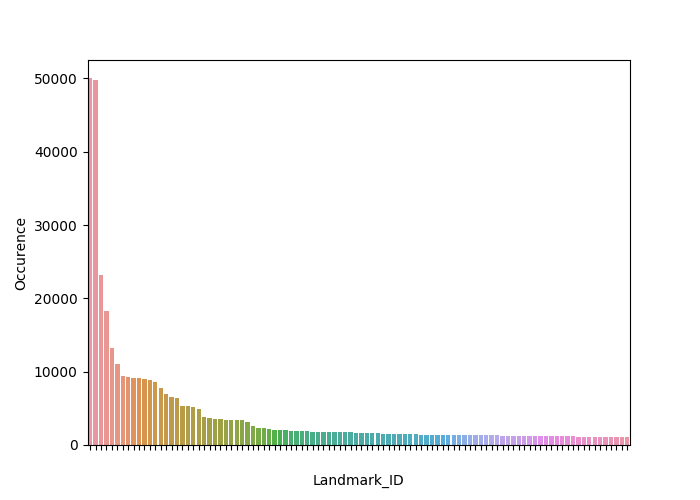
\includegraphics[width=\textwidth]{images/distribution}
	\caption{Landmark\_ID Distribution}
	\label{distribution}
\end{figure}

\begin{figure}
	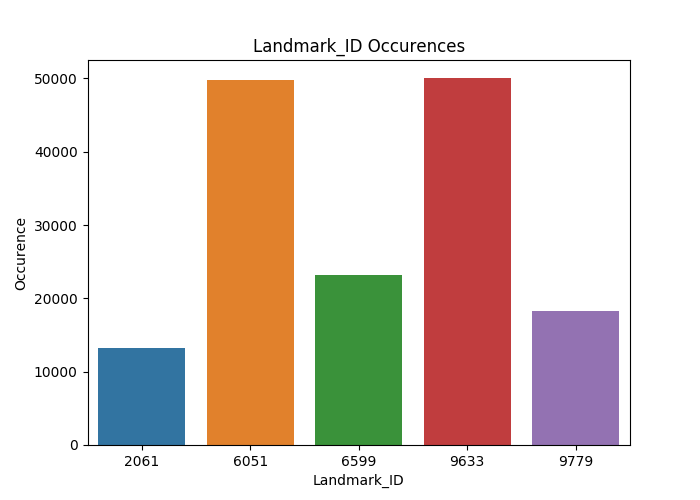
\includegraphics[width=\textwidth]{images/Landmark_ID_occurences}
	\label{landmark-ids}
\end{figure}
	
\begin{figure}
	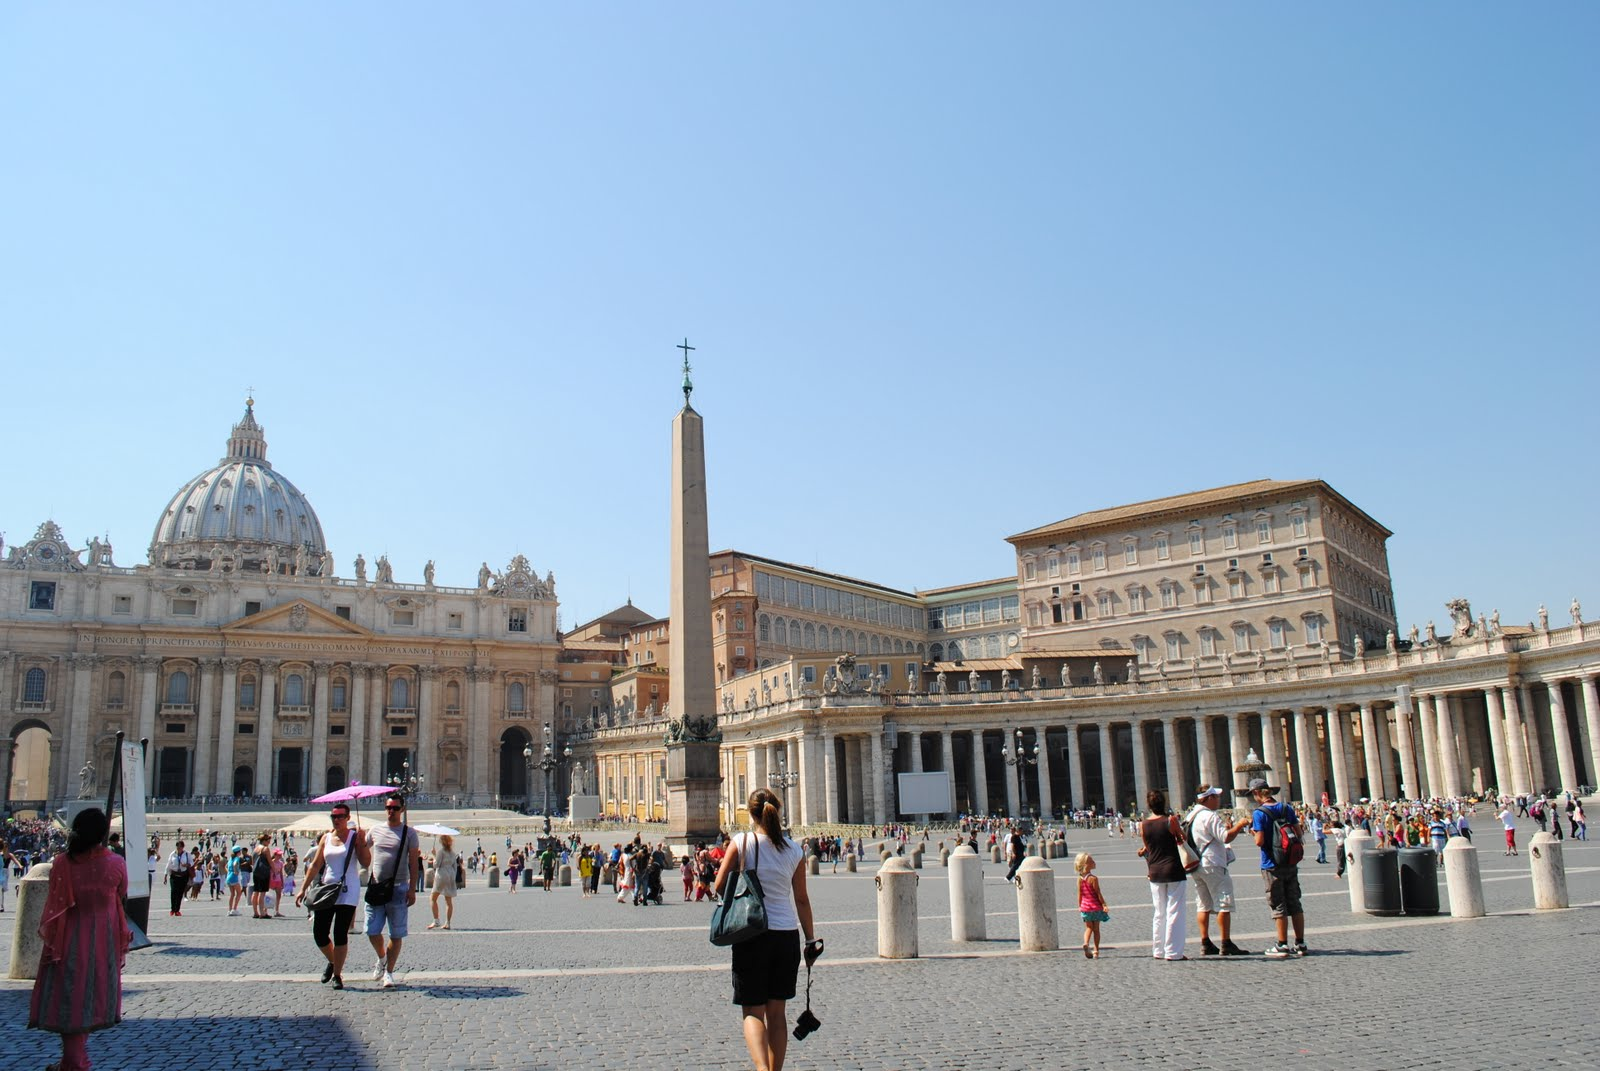
\includegraphics[width=\textwidth]{images/9633}
	\caption{Image for Landmark\_ID 9633}
	\label{9633}
\end{figure}
	
\begin{figure}
	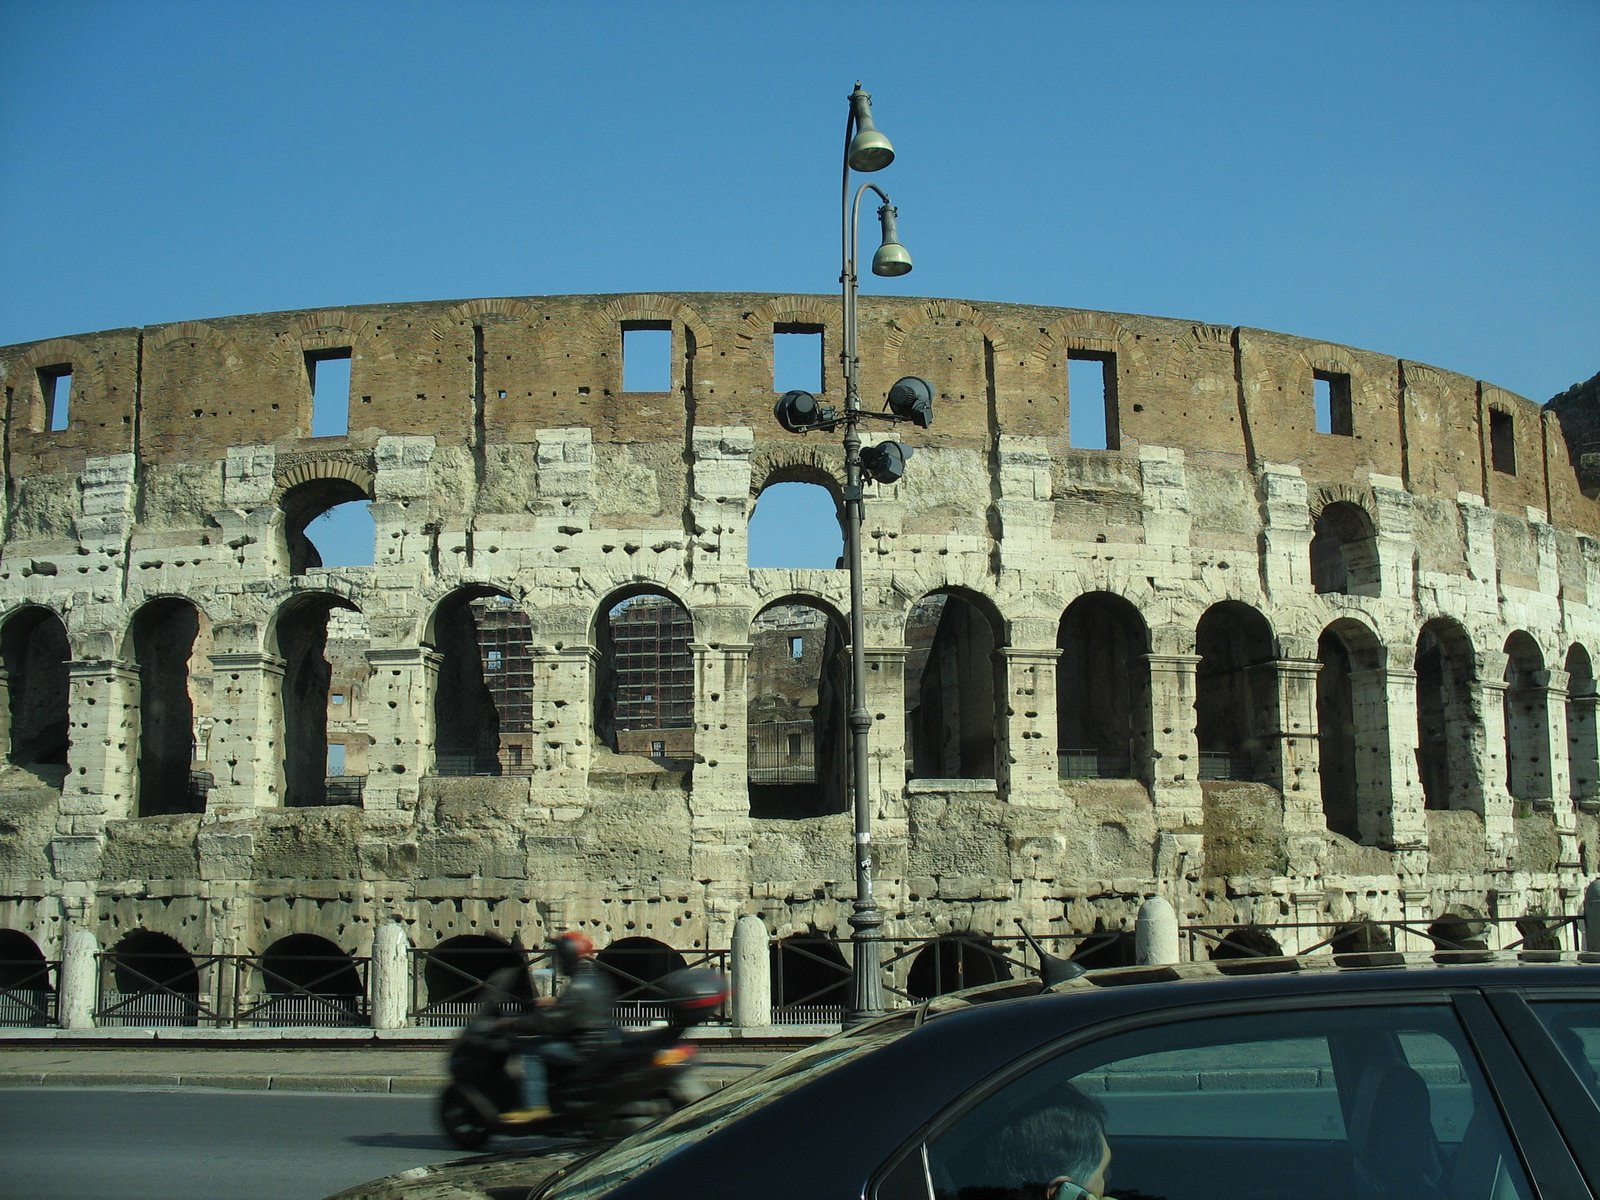
\includegraphics[width=\textwidth]{images/6051}
	\caption{Image for Landmark\_ID 6051}
	\label{6051}
\end{figure}

\begin{figure}
	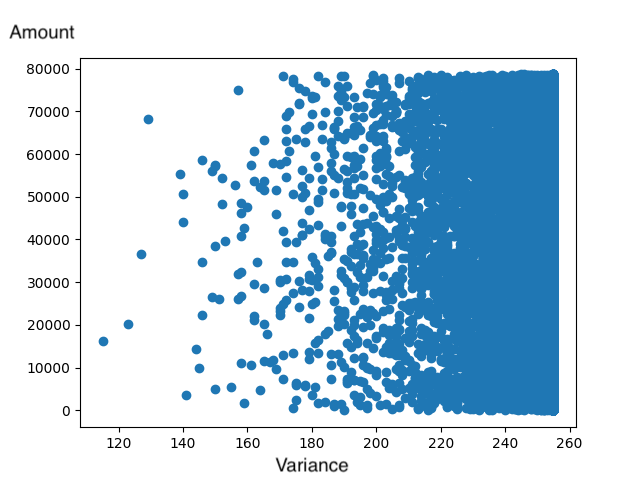
\includegraphics[width=\textwidth, height=10.5cm]{images/variances}
	\caption{Variances}
	\label{variances}
\end{figure}

\begin{figure}
	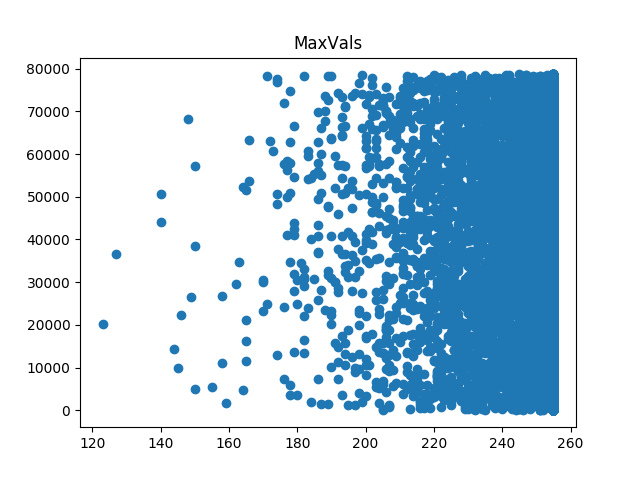
\includegraphics[width=\textwidth, height=10.5cm]{images/maxVals}
	\caption{Maximum Pixel Values}
	\label{maxVals}
\end{figure}

\begin{figure}
	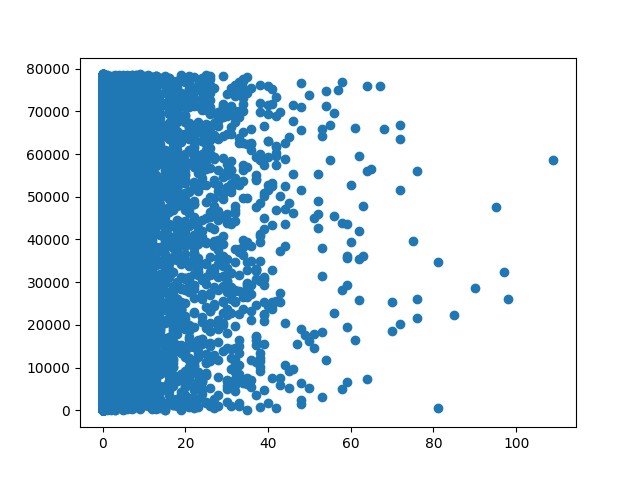
\includegraphics[width=\textwidth, height=10.5cm]{images/minVals}
	\caption{Minimum Pixel Values}
	\label{minVals}
\end{figure}

\begin{figure}
	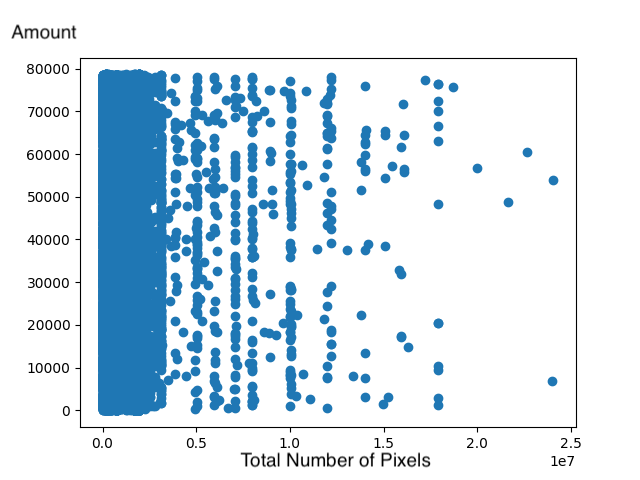
\includegraphics[width=\textwidth, height=10.5cm]{images/numPixels}
	\caption{Amount of Pixels Scatter Plot}
	\label{numPixels}
\end{figure}

\begin{figure}
	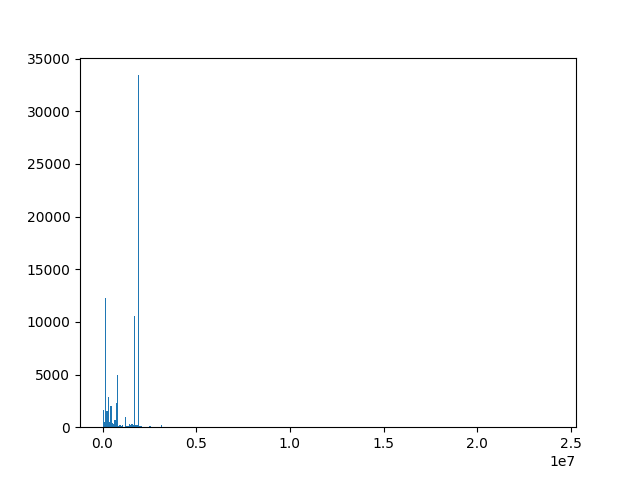
\includegraphics[width=\textwidth]{images/numPixelsHist}
	\caption{Amount of Pixels Histogram}
	\label{numPixelsHist}
\end{figure}


\chapter{Features}

For feature extraction we do a dimension reduction with PCA. For this - as a first attempt - we defined $['shape0','shape1','shape2','max','min','variance','numPixels']$ as our list x of features. 
The first three features in the list define the imgage-shape, where shape2 is the channel. The other features are as defined in section \ref{cha:data}. 
Because PCA is effected by scale we scaled the list x of features in our data with StandardScaler (sklearn)  before applying PCA.  
After standardization we  defined a number of principial components and project the seven dimension into two dimensions/ principal components. 
Together these two components contain 77\% of information (result: pca.explained\_ variance\_ ratio [0.39748574 0.37312782]).
We visualize the result of PCA with scatter (mathplotlib), which you can see in the following figure.  
\begin{figure}
	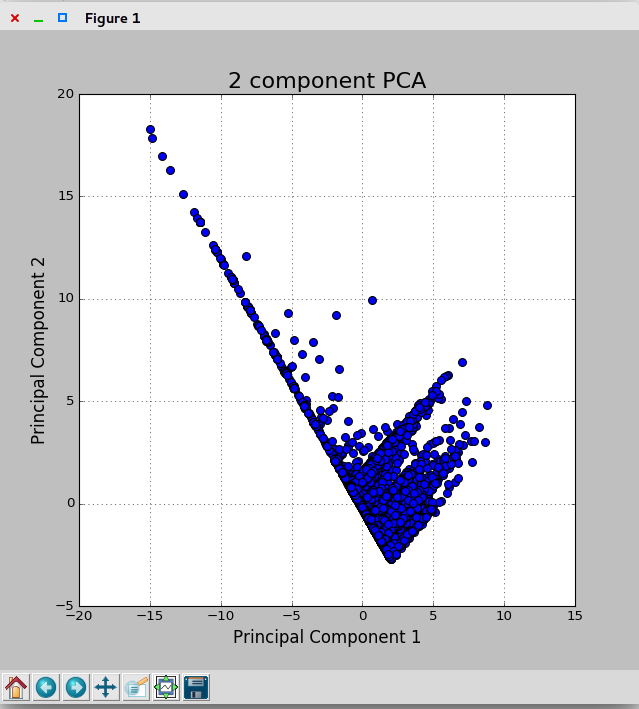
\includegraphics[width=0.7\textwidth]{images/pca}
\end{figure}

%TODO
%
%imbalances, non-normalized features
%
%extract features
%
%are they correlated
%
%cluster features with respect to correlation coefficient
%
%which features are important
%
%preprocess data
%
%cluster data (or explain why not possible) (maybe cluster only some features)
%
%dimensionality reduction method (e.g. PCA) or CNN Feature Map?

\section*{Interesting Features}

\section*{Clustering}

The clustering of the image features is a key task in this challenge. We worked out a first approach at feature extraction with the Principal Component Analysis in the previous section trying to extract the most significant features in order to leave out the unsignificant ones. This is a good way of reducing dimensions for both improved simplicity and performance. However, this is also the main task of Assignment 11 and would require too much of next week's work. Our approach is to create a feature map with a deep convolutional neural network and to classify the images with these extracted features.

\chapter{Conclusion}

The dataset is well distributed and well fitting for creating a module that can recognize landmarks in different kinds of images. The images have a various number of shapes and dimensions and are therefore a good basis for a versatile training.

Our analysis showed that a deep learning approach with a convolutional neural network is a fitting choice for this problem due to the amount of data and the difficulty of the task. We will primarily focus on a subset of the provided data for this project in order to keep the calculation time at an appropriate level.

\phantomsection % ben�tigt f�r korrekte pdf-darstellung
\addcontentsline{toc}{chapter}{References}
\bibliographystyle{natdin} % Din 1505 nach Lorenzen (Das konkrete Aussehen des Litverzeichnisses ist im header festgelegt)
\bibliography{bibliography/literatur}  % Pfad zur *.bib-Datei (Dateiendung wird weggelassen)
\cleardoublepage

\end{document}
